%%%%%%%%%%%%%%%%%%%%%%% file typeinst.tex %%%%%%%%%%%%%%%%%%%%%%%%%%%%%%
%
% This is the LaTeX source for the instructions to authors using
% the LaTeX document class SVMultln with class option 'lnicst'
% for contributions to the Lecture Notes of the Institute for
% Computer Sciences, Social-Informatics and
% Telecommunications Engineering series.
% www.springer.com/series/XXXX       Springer Heidelberg 2007/08/05
%
% It may be used as a template for your own input - copy it
% to a new file with a new name and use it as the basis for
% your article. It contains a few tweaked sections to demonstrate
% features of the package, though.
%
% If you have not much experiences with Springer LaTeX support,
% you should better use the special demonstration file "lnicst.tex"
% included in the LaTeX package for LNICST as template.
%
%%%%%%%%%%%%%%%%%%%%%%%%%%%%%%%%%%%%%%%%%%%%%%%%%%%%%%%%%%%%%%%%%%%%%%%%

%\documentclass[lnicst,sechang,a4paper]{svmultln}
%\documentclass[12pt]{llncs}
\documentclass[runningheads,a4paper]{llncs} %this is for NSS


\usepackage{amssymb}
\setcounter{tocdepth}{3}
\usepackage{graphicx}


%\usepackage{amssymb}
%\setcounter{tocdepth}{3}
%\usepackage{graphicx}
%\usepackage{fancyhdr}
%\usepackage{lastpage}

\usepackage{url}

%\urldef{\mailsa}\path|{alfred.hofmann, ursula.barth, ingrid.haas, frank.holzwarth,|
%\urldef{\mailsb}\path|anna.kramer, leonie.kunz, christine.reiss, nicole.sator,|
%\urldef{\mailsc}\path|erika.siebert-cole, peter.strasser, lncs}@springer.com|    
%\newcommand{\keywords}[1]{\par\addvspace\baselineskip
%\noindent\keywordname\enspace\ignorespaces#1}


%added by the author himself
\usepackage{color}
\usepackage[numbers]{natbib}
\usepackage{calc}
\usepackage{siunitx}
\DeclareSIUnit\mt{\milli\tesla} %% A method for say short cut or new unit!
\sisetup{inter-unit-product = {-}}

\newcolumntype{P}[1]{>{\centering\arraybackslash}p{#1}}


%added by kimmo
%\setlength\parskip{12pt}
%\setlength\parindent{0pt}
%\pagestyle{fancy}
%\fancyhf{} 
%\fancyfoot[C]{\thepage\ / \pageref{LastPage}}
%\renewcommand{\headrulewidth}{0pt}

\begin{document}

\mainmatter  % start of an individual contribution

% first the title is needed
\title{Concealing IMSI in 5G Network Using Identity Based Encryption}
%Concealing IMSI in 5G Network Using Identity Based Cryptography

% a short form should be given in case it is too long for the running head
\titlerunning{Concealing IMSI Using Identity Based Encryption} 

% the name(s) of the author(s) follow(s) next
%
% NB: Chinese authors should write their first names(s) in front of
% their surnames. This ensures that the names appear correctly inlso
% the running heads and the author index.
%
\author{Mohsin Khan%
%%\thanks{Please note that the LNICST Editorial assumes that all authors have used
%%the western naming convention, with given names preceding surnames. This determines
%%the structure of the names in the running heads and the author index.}%
\and Valtteri Niemi\\
\email{mohsin.khan@helsinki.fi, valtteri.niemi@helsinki.fi}
}  %

\authorrunning{Mohsin Khan \and Valtteri Niemi}
% (feature abused for this document to repeat the title also on left hand pages)

% the affiliations are given next
\institute{University of Helsinki, Department of Computer Science,\\
P.O. Box 68 (Gustaf H\"allstr\"omin katu 2b)\\
FI-00014 University of Helsinki\\
Finland\\
\url{https://www.cs.helsinki.fi/en}
}

%relationship stu
%
% NB: a more complex sample for affiliations and the mapping to the
% corresponding authors can be found in the file "lnicst.dem",
% that is contained in the LNICST LaTeX support package.
%

%%%\toctitle{Lecture Notes in Computer Science}
%%%\tocauthor{Authors' Instructions}
\maketitle


\begin{abstract}
The aspirations for the next generation mobile network (5G) are high. It has a vision of improved security and privacy compared to the existing LTE network. Subscription privacy of a user has been a historical concern with all the previous generation mobile networks, namely, GSM, UMTS, and LTE. While a little improvement have been achieved in securing the privacy of the long-term identity of a subscriber, the so called IMSI catchers are still in existence even in the LTE and advanced LTE networks. Proposals have been published to tackle this problem based on pseudonyms, and different public-key technologies. This paper looks into the problem of concealing long-term identity of a subscriber and presents a technique based on identity based encryption (IBE) to tackle it. In addition to protecting identity privacy, the proposed solution can be extended to a mutual authentication and key agreement protocol between a serving network (SN) and a user equipment (UE). This mutual authentication and key agreement protocol runs only between the SN and the UE  and does not need to connect with the home network (HN) on every run. A rigorous comparison of the advantages and disadvantages of different techniques show that IBE based solution is a competitive solution for securing the long-term identity privacy of a user in the 5G network.
\end{abstract}


\section{Introduction}
\label{intro} The NGMN Alliance has pointed out the privacy of a user as a requirement of the 5G network \cite{NGMN_white_paper}. When a user equipment (UE) tries to connect to a network, the UE has to identify itself using an identifier. Once the UE is identified, an authentication protocol is run between the UE and the network. If the authentication protocol ends successfully, the network serves the UE with the services the UE is authorized to avail. There are two types of attackers against the user privacy. A passive attacker just listens to the radio communication and tries to figure out identity of the user. An active attacker may transmit some radio messages itself. It is much easier to protect against a passive attacker than against an active attacker. Since 2G (GSM) the network has used temporary identities to protect against passive attckers. On the other hand, even in the LTE network the permanent identity is not protected against active attackers.

We discuss solutions to conceal the long-term identifier known as international mobile subscriber identity (IMSI) during the identification phase. These solutions are based on pseudonyms and public-key encryption. The pseudonym based approaches require to maintain a synchronization of pseudonyms between the UE and the HN. It may be difficult to resynchronize the pseudonyms once the synchronization is lost. We discuss solutions based on certificates and root-key for the category of public key based solutions. Unlike the pseudonym based solutions these public-key based solutions do not require any synchronization. On the other hand, the public-key based solutions have higher cost both in terms of communication and computation. 

Then, we also propose a novel solution based on identity based encryption (IBE). One additional advantage of our solution is that, it also works as a mutual authentication protocol between SN and UE without the involvement of the HN every time the authentication is needed. This additional advantage can not be achieved using root-key based approach. Even though the additional advantage can be achieved using certificates, the certificate based approach is the heaviest in terms of communication and computational complexity.

Apart from preventing the attackers, there are other 5G requirements which a solution should also meet. An IMSI includes the identity of a user along with the identity of the user's home network. It may be required to conceal the identity of both the network and the user. Reduced signalling overhead, improved control plane latency are also important requirements. In the case of public-key, the complexity involved in setting a PKI and revocation of a public-key need to be considered with high importance. In some cases the public key of an entity is pre-provisioned to all the potential senders in the system. If this public key is revoked and a new public-private key pair is generated by the entity from which the public key was revoked, then the new public key needs to be re-provisioned to all those entities that were pre-provisioned with the old public key. Considering these requirements, we evaluate our solutions based on the following criteria: (1) Immunity to attackers, (2) Parts of the IMSI concealed, (3 ) Signalling overhead, (4) Latency, (5) PKI complexity, (6) Public-key revocation, etc. While the choice of the solution is dependent on how much we want to achieve, our solution based on IBE becomes a competitive one by meeting most of the important requirements.

In section \ref{sec:3GPP-defined_aspects_of_mobile_network}, we introduce the necessary aspects of 3GPP defined networks that we would need to discuss the problem and solutions in a comprehensible manner. In Section \ref{sec:existing_solutions} we present high-level discussions of different published solutions based on pseudonyms and different kinds of public-key encryption. In section  \ref{sec:solutions_based_on_IBE}, we present a solution based on IBE that is not only identification but also works as mutual authentication. In Section \ref{sec:evaluation}, we present a comparison of the discussed solutions along with our proposed solution based on different evaluation criteria. Finally we conclude the paper in Section \ref{sec:conclusion}.

\section{3GPP-defined Aspects of Mobile Networks}
\label{sec:3GPP-defined_aspects_of_mobile_network}
The 3rd Generation Partnership Project (3GPP) unites seven telecommunications standard development organizations (ARIB, ATIS, CCSA, ETSI, TSDSI, TTA, TTC), known as Organizational Partners (OP) and provides their members with a stable environment to produce the Reports and Specifications that define 3GPP technologies \cite{3gpp_intro}. Contributions of the members are documented in the technical report (TR) documents first. Useful and feasible contributions in the TR documents eventually become the specifications and make their way to the technical specification (TS) documents. 

In 3GPP TR 33.899 \cite{TR33899}, subscribers' privacy is captured as one of the high level security requirements of the 5G network. However, in the context of diversified devices and the complex business and service model of 5G, it is important to define who is a subscriber and what subscriber privacy means. According to 3GPP TR 21.905 \cite{TR21905}, a subscriber is an entity (associated with one or more users) that is engaged in a subscription with a service provider. A subscription describes the commercial relationship between the subscriber and the service provider, cf. 3GPP TR 21.905 \cite{TR21905}. A subscription identifier is the identifier that uniquely identifies a subscription in the 3GPP system. The identifier is used to access networks based on 3GPP specifications. Subscription privacy refers to the right to protect any information that (a) can be used to identify a subscription to whom such information relates, or (b) is or might be directly or indirectly linked to a subscription. This definition of privacy suggests to protect any personally identifiable information (PII) from an attacker. While it may be difficult to draw a clear boundary between PII and non-PII, the long-term identifier is surely a PII. 

\subsection{System Overview}
In the case of GSM, 3G (UMTS) and 4G (LTE) networks, IMSI is a long-term identity of a subsriber. An IMSI is usually presented as a $15$ digit number but can be shorter. The first $3$ digits are the mobile country code (MCC), which are followed by the mobile network code (MNC), either $2$ digits or $3$ digits. The length of the MNC depends on the value of the MCC. The remaining digits are the mobile subscription identification number (MSIN) within the network's customer base \cite{TS23003}. 

In order to present an easily comprehensible formal discussion, we need to know what are the entities involved in this identification process and what are the communication interfaces between those entities. We also need to know which entities can be entrusted with the IMSI of a subscriber. As the architecture of 5G is yet to be finalized, we present an abstraction of the involved entities and assume that whatever the architecture of 5G will eventually be, it will contain something for each of these entities and something for each of these interfaces. This abstraction is directly extracted from the LTE architecture. Figure \ref{fig:security_architecture_abstraction} shows the abstraction.

The abstraction involves the UE, SN and HN. Both of the SN and HN consist of radio access network (RAN) and core network (CN). The RAN of SN provides the connectivity between UE and CN of SN. On the other hand, the CN of SN connects itself with the CN of HN. However, we do not present such granularity of SN and HN, because in our discussion it is sufficient to treat the SN and HN as single abstract entities. Note that in a non-roaming situation, the SN and HN are the same network. There are two more entities which are not part of the network but relevant in our discussion, because they attack the network. They are passive IMSI catcher (PIC) and active IMSI cather (AIC). 

The interface UE-SN is a logical interface between UE and SN. This interface is initially unprotected. The logical interface SN-HN between SN and HN is protected and the security of this interface is out of the scope of this paper. The PICs eavesdrop on the UE-RAN interface when it is unprotected to extract an IMSI. The AICs impersonate a legitimate SN and run a legitimate looking protocol with the UE in order to find out the IMSI. 


HN and UE both know the IMSI and they are trusted. Both of PIC and AIC are untrusted. It is in principle possible not to trust SN. However, by other specifications in 3GPP TS 33.106 \cite{TS33106} and TS 33.107 \cite{TS33107}, it is required to reveal IMSI to the SN to enable lawful interception (LI) without involving HN. \begin{figure}

\begin{center}
% Use the relevant command to insert your figure file.
% For example, with the graphicx package use
  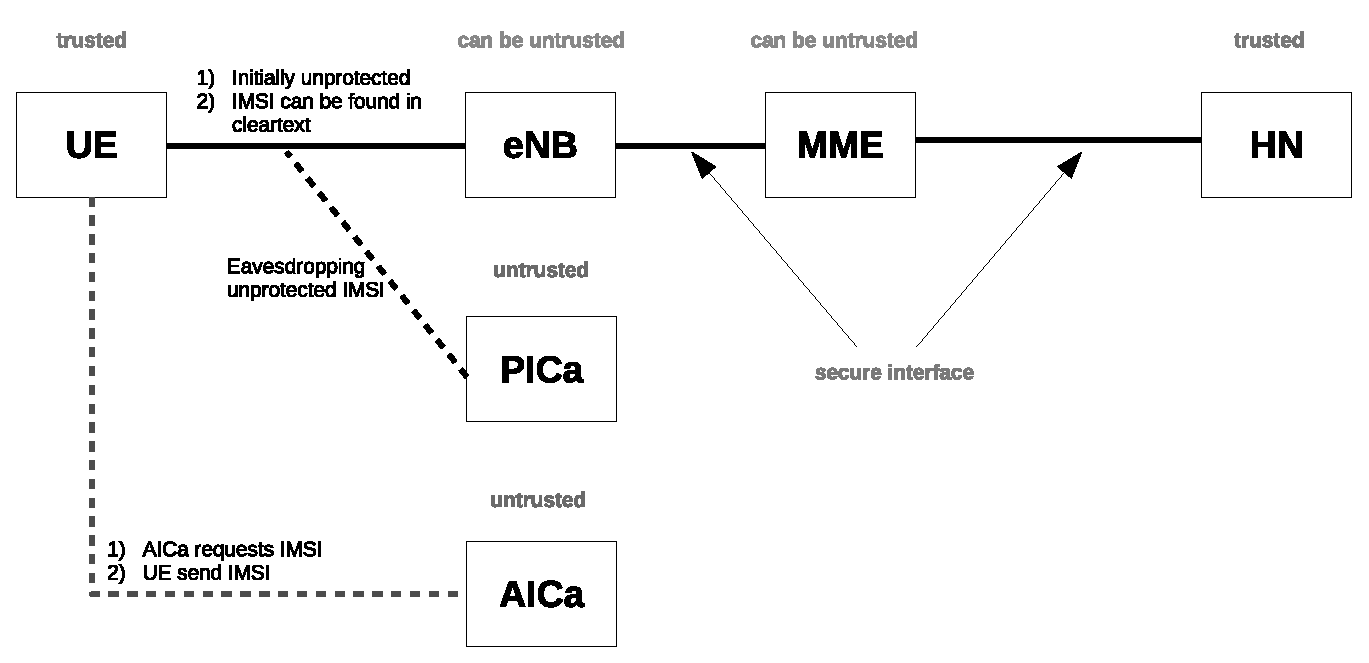
\includegraphics[height= 5cm]{security_architecture_abstraction.eps}
% figure caption is below the figure
\caption{High-level security architecture}
\label{fig:security_architecture_abstraction}       % Give a unique label
\end{center}
\end{figure} 

\subsection{Current Solution Approach and its Weakness}
One approach of protecting IMSI privacy is to use a temporary identifier instead of the actual IMSI and keep changing the temporary identifier at a feasible frequency. Note that the temporary identifier has to be assigned over a confidentiality protected channel and different entities of the network may assign different temporary identifiers to the UE. 

In the LTE network, the temporary identifier assigned by a serving network (SN) is called globally unique temporary identity (GUTI) and the home network (HN) does not assign any temporary identifier to the UE. However, during the initial attachment of a UE to the SN, the UE has neither a GUTI nor a security context with the SN that can assign it with a GUTI. Besides, GUTI can be lost by either one or both of the UE and the SN. This would force the UE to reveal its IMSI to the SN to keep itself from permanently locked out of the network.

This problem gives an opportunity to an AIC who impersonates a legitimate SN and forces the UE to run the initial attachment protocol. This also gives an opportunity to a PIC to eavesdrop the IMSI sent in clear text. Solutions \cite{pseudonym_valtteri_philip, pseudonym_ericsson} have been proposed by using temporary IMSI known as pseudonym assigned by the HN. While these solutions solve the cases of lost and unsynchronised GUTI, they still have the problem of lost or unsynchronised pseudonyms and also initial attachment. Public-key technologies have also been considered as potential approach to solve this problem




\section{Discussion on Different Proposed Solutions}\label{sec:solutions} 
\label{sec:existing_solutions}
Different solution techniques have been published to prevent the AICs. In this section we will discuss on those solutions on a high level. Before delving into those solutions, let us introduce some notation. 
\begin{enumerate}
\item $hnid=MCC||MNC$ identifies the HN
\item $snid=MCC||MNC$ identifies the SN
\item $e_A$ is the public key of entity $A$
\item $d_A$ is the private key of entity $A$ 
\item $\mathcal{X}_{A,B}(e_A,e_B)$ is the certificate of the public key $e_A$ of $A$. The certificate can be verified by anyone who considers $B$ as a root CA using the public key $e_B$. The certificate is a guarantee from B that the public key $e_A$ is owned by $A$ .
\item $E,D$ are the encryption and decryption functions so that $D(E(M,K),K) = M$.
\item $S(M,K)$ is the signature of message $M$ signed by the key $K$
\end{enumerate}

\subsection{Solution Based on Pseudonyms:}
\label{sec:pseudonyms}
Pseudonym based solutions have been proposed in \citep{pseudonym_ericsson,pseudonym_valtteri_philip}. In this kind of solutions, the HN assigns a temporary identifier called pseudonym to a UE. Next time when the UE tries to identify itself to an  SN, it uses the pseudonym instead of IMSI. Periodically, whenever there is an opportunity, the HN sends a new pseudonym to the UE with confidentiality and integerity protection. One such opportunity could be when the HN sends the authentication vector to an SN.

\subsection{Solution Based on Certificate Based Public-key Cryptography} 
\label{sub_sec:solution_certificate}
Use of certificate based public-key encryption to conceal long-term identity has been suggested in 3GPP TR 33.821 \cite{TR33821}. To use certificate based public-key cryptography for securing IMSI privacy, we need to figure out a few things first: who are the root CAs and who else can be a CA, who are the entities that own a public key, how a certificate can be revoked, and how the UE can be re-provisioned with a new root certificate if needed. Different solutions can be devised based on the choice of root CAs and other CAs. All those solutions will require an SN to have a valid certificate that a UE can verify using a public-key that the UE trusts. Consequently the root public-key has to be provisioned to all the UEs. An SN has to obtain a certificate verifiable by all the UE the SN intends to serve. We provide a high-level description for few candidate variants of certificate based solution.

\subsubsection{Variant 1:}
It uses a global root of trust. There is a global entity trusted by everyone. Using this trusted global entity, a chain of trust can be established. The SN presents the certificate to a UE trying to attach. The UE verifies the certificate. If the verification result is positive, the UE encrypts its IMSI using the public key of the SN and sends to the SN. Thus the entire IMSI is concealed from both the AIC and PIC.

\subsubsection{Variant 2:}
In this variant the HN of a subscriber acts the root CA for the subscriber. In this case, the HN generates a public-private key pair and generates a certificate of the public key signed by the HN itself. A UE is provisioned with this self signed certificate. An SN interested to serve a UE obtains a certificate from the UE's HN. SN sends its public key $e_{snid}$ and $snid$ to the HN. The HN generates a certificate $\mathcal{X}_{snid,hnid} (e_{snid},e_{hnid})$. When the SN broadcasts its identity, the UE sends $hnid,e_{hnid}$ to the SN. The SN looks up for the certificate $\mathcal{X}_{snid,hnid} (e_{snid},e_{hnid})$. In case it exists at the disposal of the SN, the SN sends $\mathcal{X}_{snid,hnid} (e_{snid},e_{hnid})$ to the UE. The UE verifies the certificate and extracts the public key $e_{snid}$ from the certificate. If the certificate is verified as valid, then the UE sends the IMSI to the SN encrypted by the public key $e_{snid}$ of the SN.  Note that the SN does not need to get the certificate from the HN, but the SN can get it from any CA who is trusted in by the HN in the chain of trust. 

\subsubsection{Variant 3:}
In this variant, there is no other CA than the root CA. Hence the chain of certificates is very short. Only an HN can be a CA. The certificates of all the SNs a UE might visit are pre-provisioned to the UE by the HN. When a UE attempts to attach to an SN, the UE encrypts the IMSI with the public key of the SN which is already provisioned to the UE. If the public key of an SN is revoked, the HN has to provision the revocation to the UE.


\subsection{Solution Based on Root-key based Encryption} 
\label{sub_sec:solution_root-key}
In root-key based public-key encryption, there is only a very limited number of public-private key pairs in the network. All the senders in the network are pre-provisioned with the public key of the receivers. We use only one pair of public-private key pair in this approach. Such a technique has been proposed in 3GPP TR 33.899 in solution \#7.3. This key pair is owned by the HN and we call it to be the root-key. The HN provisions the public key to all the UEs that have subscriptions with the HN.  Whenever a UE is in need of identifying itself to an SN with the IMSI, the UE encrypts the IMSI with the public root key and sends the result to the SN along with the $hnid$. The SN sends the encrypted IMSI to the appropriate HN. The HN then decrypts and extracts the IMSI. The HN sends the IMSI back to the SN. HN decrypts and extract the IMSI. HN sends back the IMSI to the SN along with an authentication vector (AV) that is used for running an authentication protocol between the UE and the SN.

\subsection{Solution Based on IBE}
In the next section we discuss the basic principles of IBE and present a solution of the identity privacy using IBE. The solution is extended to a mutual authentication and key agreement protocol.


\section{Details of the IBE Based Solution} 
\label{sec:solutions_based_on_IBE}
\subsection{How IBE works}
The idea of IBE was proposed by Adi Shamir in 1984 \cite{IBE_shamir}. In IBE, the public and private keys of a receiver are computed from the identity of the receiver in conjunction with the public and private key of a trusted third party respectively. A sender does not need to authenticate the public key of a receiver each time the sender and the receiver agree on a security context. The sender does not need to authenticate the public-key, because if the public key is not authentic, the receiver will not have the private key. If the receiver does not have the private key, any message encrypted by the public key will never be decrypted by the receiver. On the other hand, the private key of the receiver would be provisioned to the receiver only if the receiver can authenticate itself to the trusted third party. In other words, the authenticity of the public key in IBE is guaranteed by the trusted third party. 

Usually in IBE, the trusted third party is known as the private key generator (PKG). As the private key of the PKG is required to compute the private key of the receiver, the private key of the receiver has to be provisioned to the receiver by the trusted third party. While in the certificate based and root-key based solutions it is possible to revoke the public key of a receiver, it is impossible to revoke the public key in IBE unless the identity itself is revoked. Please note that a PKG knows the private keys of all the receivers whose public keys were generated using the PKG's public key. As a result a PKG can decrypt any message sent by any sender to any receiver. This implies that there must be a very high level of trust in the PKG.

Dan Boneh and Matthew Franklin published a fully functional IBE scheme in 2003 \cite{IBE_boneh_franklin}. The security of this
scheme was based on a natural analogue of the computational Diffie-Hellman assumption. Based on this assumption they showed that the new system has chosen ciphertext security in the random oracle model. To make the revocation of public keys easier, this scheme also suggests to use an expiry time as part of the identity of a receiver. We use this suggestion in our solution. Clifford Cocks present an implementation in 2001 \cite{IBE_clifford} and show that the security of the implementation is related to the difficulty of solving the quadratic residuosity problem.


\subsection{Existing proposals of Using IBE in 5G Network}
RFC 6508 \cite{RFC6508} presents an algorithm SAKKE for establishment of a secret shared value. Applications of SAKKE may include a date-time component in their identity to ensure that identities and hence the corresponding private-keys are only valid for a fixed period of time. Solution \#7.11 in 3GPP TR 33.899 \cite{TR33899} uses IBE to protect the long-term identity according to RFC 6508. However, the solution does not address the issue of revocation of the identity based public-keys. RFC 6507 \cite{RFC6507} describes a certificate-less signature scheme based on IBE. In this scheme a string called public validation token (PVT) randomly chosen by the PKG is assigned to an identity. Both the public and private key of a receiver are computed using the PVT along with the receiver's identity. So, the public key associated with an identity can be revoked by revoking the PVT. Solution \#2.14 in 3GPP TR 33.899 presents an authentication framework based on the signature scheme of RFC 6507 and the authentication protocol EAP-TLS. This solution uses the PVT to revoke the public key associated with an identity. However, in this solution it is not clear how a UE can check if the public key of an SN has been revoked or not.

\subsection{The Proposed Solution}
Next we present a protocol that serves the purposes of both privacy protected identification of UE and mutual authentication between UE and SN. This mutual authentication does not require a contact with the HN each time the protocol is run between a UE and an SN. In our solution we do not use PVT but instead use an expiry time with pre-agreed format. This expiry time can act as the PVT. If the public key of an identity needs to be revoked, the expiry time along with the identity is added to the revocation list. If the identity requires a new public key, the PKG uses another expiry time to compute the private key of the identity. The newly computed private key is then provisioned to the identity along with the the new expiry time. When the expiry time comes, all the public keys computed using the expiry time are automatically revoked. So, the revocation list does not need to include revocations whose expiry time is in the past.


\begin{figure}
\begin{center}
% Use the relevant command to insert your figure file.
% For example, with the graphicx package use
  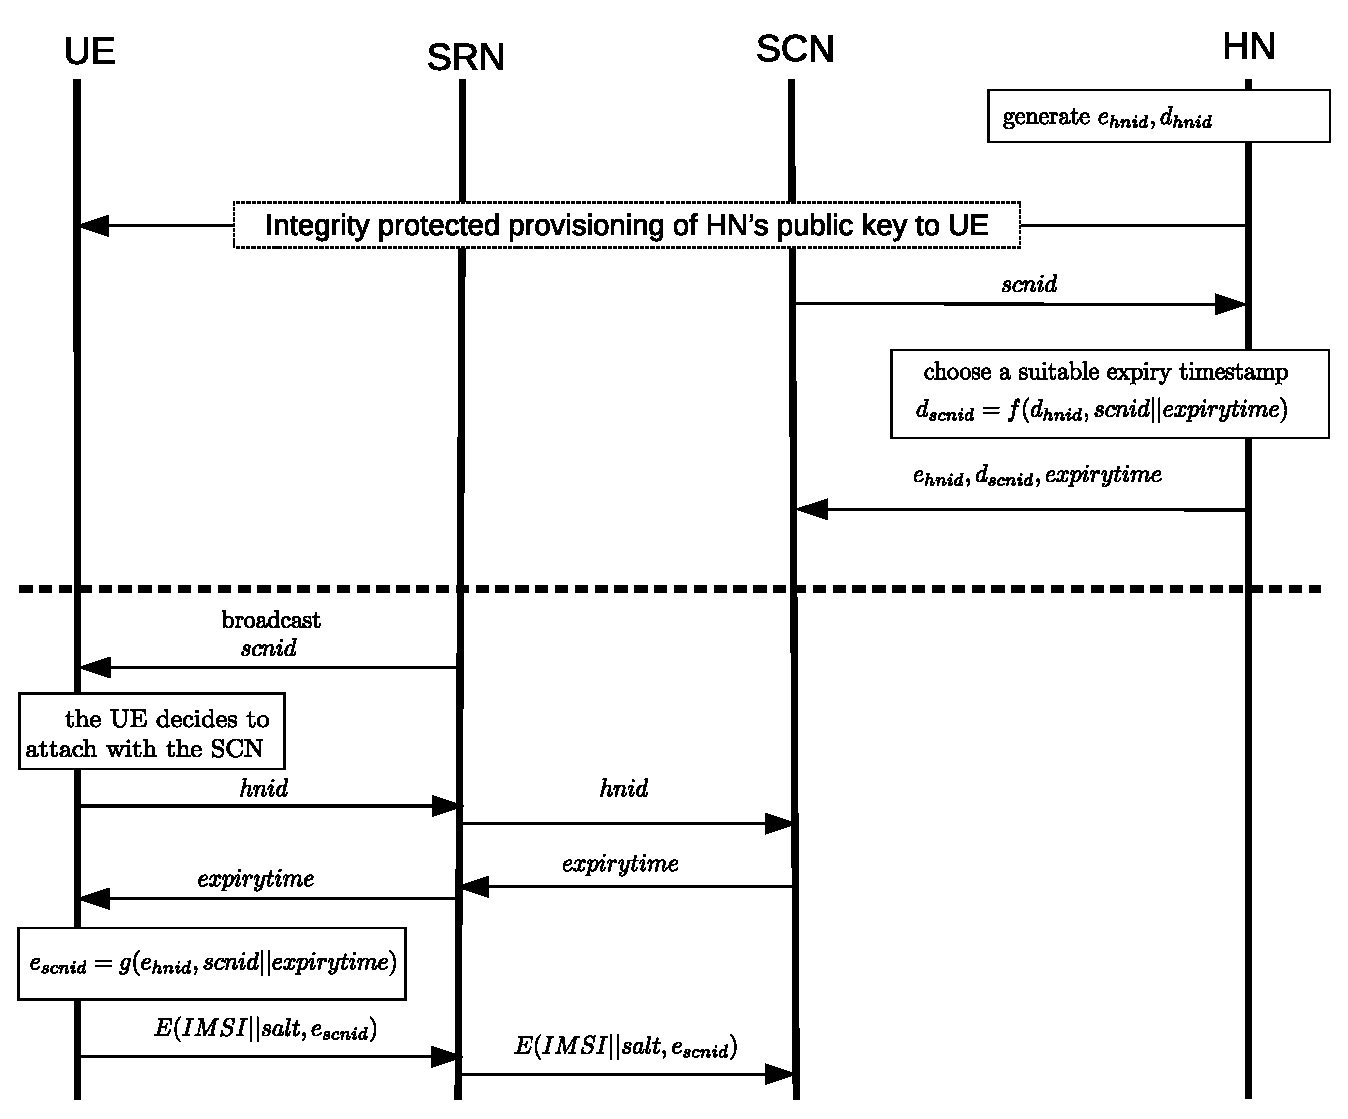
\includegraphics[height=7cm]{solution_based_on_ibc.eps}
% figure caption is below the figure
\caption{Privacy protected UE identification and mutual authentication using IBE}
\label{fig:solution_ibc}       % Give a unique label
\end{center}
\end{figure}

\subsubsection{Description of the proposed solution}
The UE's HN acts as the PKG. The solution is pictorially presented in Figure \ref{fig:solution_ibc}. It has two different phases. In the first phase, the key generations and provisioning take place. In the second phase the identification and authentication happens. The steps in the first phase are identified by $1.*$ and by $2.*$ in the second phase. The description follows:

\begin{itemize}

\item The HN generates a public-private key pair $e_{hnid},d_{hnid}$ in step $1.1$. 

\item In step $1.2$, the HN provisions the UE with the public key $e_{hnid}$ and the private key $d_{ue}$. The private key $d_{ue}$ is generated using the private key $d_{hnid}$, $IMSI$, and a chosen expiry time $ET_{eu}$. 

\item The SN sends the $snid$ to HN in step $1.3$. 

\item In step $1.4$ the HN chooses a suitable expiry time $ET$ to generate the private key of the SN. The expiry time is appended with $snid$ and the private key $d_{snid}$ is computed considering $snid||ET$ as the identity of the SN. 

\item In step $1.5$, the HN sends $d_{snid}$ to the SN along with $ET$ and $e_{hnid}$. The SN stores these information in its key-table. 

\item In step $2.1$, the SN broadcasts the $snid$. 

\item In step $2.2$ the UE sends $hnid,E(IMSI||ET_{ue}||RAND1,e_{snid}),ET$ to the SN. 

\item In step $2.3$ the SN looks for an appropriate private key $d_{snid}$ compatible with $ET$. 

\item If SN has such a private key then it jumps to step $8$. Otherwise it continues from step $2.4$ and stop at step $2.7$. 

\item In step $2.4$ SN sends $snid,E(IMSI||ET_{ue}||RAND1),ET$ to HN. 

\item In step $2.5$ HN computes the key $d_{snid}$ using $d_{hnid},snid$ and $ET$. Then HN decrypts the received encrypted message using the key $d_{snid}$. After extracting the the IMSI from the decrypted message, HN prepares an $AV$ that can be used in EPS-AKA. 

\item In step $2.6$, HN sends the $AV$ along with the $IMSI$ and $d_{snid}$. The SN stores $d_{snid}$ along with the $ET$. 

\item In step $2.7$ EPS-AKA is run between UE and SN and consequently mutual authentication and key agreement is achieved.

\item However, if SN finds an appropriate $d_{snid}$ in step $2.3$, then the protocol jumps to step $2.8$. In step $2.8$ SN decrypts the received encrypted message and compute $e_{ue}$ using $IMSI||ET_{ue}$ and $e_{hnid}$. 

\item In step $2.9$ HN sends the signature $S(IMSI||RAND1||RAND2,d_{snid})$ along with $E(RAND2,e_{ue})$ to the UE. The signature is verifiable by $e_{snid}$ in the UE. 

\item In step $2.10$ the UE sends the signature $S(IMSI||RAND1||RAND2,d_{ue})$ to the SN which is verifiable by $e_{ue}$. If both UE and SN can verify the signatures as valid, the mutual authentication is completed successfully.

\end{itemize}

Note that UE and SN have successfully exchanged two randomly chosen values RAND1 and RAND2 with confidentiality protection. A symmetric key can be computed at both UE and SN using these random values and $e_{hnid}$ using a function like key derivation function used in LTE security. There is also an alternative option of using ephemeral Diffie-Hellman key exchange protocol. The messages required for the ephemeral Diffie-Hellman key exchange can be transported along with the messages sent in step $2.9$ and $2.10$. In that case, confidentiality protection of $RAND2$ is not required. In solution \#2.14 in 3GPP TR 33.899, a static Diffie-Hellman key exchange have been proposed. In the static Diffie-Hellman technique the public key credentials used are the same as used in the IBE based solution. Consequently, static Diffie-Hellman does not require any extra communication for the symmetric key exchange.

\subsubsection{Revocation of Public Keys}
As the public key in IBE can not be revoked, we use the concept of expiry time as the part of the identity of an entity. The expiry time is a time stamp in the future and acts as a PVT. So, when a public key needs to be revoked, the corresponding identity and expiry time is put in a revocation list. 

Any sender encrypting a message using a public key should first check in the revocation list if the relevant identifier and expiry time is revoked or not. But for a UE it is not possible to access the revocation list because it does not yet have a security context with the SN. To circumvent this problem, HN gives the private key $d_{snid}$ to an SN for a short period of time, for an example, until the day end. So, if the public key needs to be revoked, it would automatically be revoked when the expiration time comes. In this way, a compromised SN would be able mount an attack only for a short period of time. However, the SN would need to get new $d_{snid}$ from the HN before the old $d_{snid}$ expires. 

When the public key of a UE is revoked, the IMSI and relevant expiry time is stored in a revocation list in the HN.  An SN serving UEs of an HN has a copy of the list. The SN also periodically checks with the HN if there is any new revocations. Before computing the public key of the UE in step $2.8$, the SN checks the revocation list if the pair $IMSI,ET_{ue}$ is revoked or not. If it is revoked, the SN discards the message received from the UE and the authentication fails. 

As revocation of the public key of a UE is possible to be checked in a revocation list, UEs can be given private keys associated with expiry time which is fairly ahead in future, e.g., for a year. And all the entries with expiry time older than current date-time be removed from the revocation list, hence the revocation list will not grow to a very large size. This frequent private key exchange and refreshing the revocation list would create a bit increased traffic between an SN and HN. On the other hand, this increased traffic is not in the air interface but in the back haul network, which apparently is not very critical. 


\section{Comparison of Solutions}
\label{sec:evaluation}
In this paper we have discussed two different categories of solutions. One is pseudonym based and the other is public-key based. We have discussed the pseudonym based approach on a high level. Different solutions could be devised following this approach. It is reasonable to assume that all those soulutions would require the UE and the HN to synchronize their states and the used pseudonyms. Besides, if pseudonyms get lost either by the UE or the HN, the UE has to reveal its IMSI to keep itself from locked out of the network permanently or even temporarily in emergency. So, it seems public-key technology is necessary to ensure the long-term identity privacy of a subscriber. 

We have looked into different kinds of public-key technologies that serve the purpose of concealing long-term identity of a user. We have categorized the different public-key technologies into three categories: certificate based, root-key based and identity based. We have discussed three variants of certificate based solutions from a high level. We also have discussed one root-key based solution. One good side of all of these solutions is that, none of them require to maintain synchronization of states between UE and HN. But these solutions have some downsides also. All public key based technologies need comparatively heavier computational resources and the ciphertexts are longer. This heavier computation and longer ciphertexts affect the latency. Solutions based on public-key technologies also require a mechanism of key revocation. Apart from the common downsides, there are other downsides in these public-key based solutions.

In certificate based solutions there is a need of a global PKI. However, in some variants of certificate based solutions, the effort to manage a PKI can be reduced significantly. Certificate based solutions require an extra round trip between the UE and SN to exchange and verify the certificate. In a variant of a certificate based solution, this extra round trip could be removed at the expense of provisioning the certificate of an SN to a UE before the UE goes roaming to the SN. All the certificate based solutions have the requirement of exchanging certificates and verifying them. This creates signalling and computational overhead which consequently affect the latency. 

The root-key based solution does not require any extra round trips or certificates, hence it has better signalling and computational overhead compared to certificate based. However, the root-key based solution still suffers from the increased latency in a roaming situation because every authentication needs to travel all the way to the HN. This is because no one else except the HN can decrypt the message sent by the UE. The solution creates also computational pressure in the HN. It is desirable to have an authentication protocol that can run between a UE and the SN, without any involvement of the HN, thus achieving low latency in the roaming case.

We find IBE a tempting approach to solve the problem of long-term identity privacy. Different solutions based on IBE could be devised. We have proposed a novel solution based on IBE that can both accomplish the identification and mutual authentication. The solution does not need to maintain synchronized states between a UE and the HN. The solution does not require a global PKI and does not need certificates. Unlike the root-key based approach, our solution does not need to involve HN each time authentication is needed. The aforementioned argument makes the IBE based solution a potential candidate to solve the problem in question. In the below table we present a comparison among the different solutions based on different criteria.

\begin{table}
\begin{center}
\begin{tabular}{ |p{3.5cm}|P{1.25cm}|P{1.25cm}|P{1.25cm}|P{1.25cm}|P{1.5cm}| P{1cm} | }
\hline
\textbf{Criteria} & \textbf{Pseudo} & \textbf{CertV1} & \textbf{CertV2} & \textbf{CertV3} & \textbf{Root-key} & \textbf{IBE}\\
\hline \hline
Immunity to AIC & + - & + & + & + & + & + \\ \hline
Concealing $hnid$ & - & + & - & - & - & - \\ \hline
Signalling overhead & + + & - & - & - & + & + \\ \hline
Computational overhead & + & - & - & - & + & + \\ \hline
Latency while roaming & - & - & -  & - & - & + \\ \hline
Latency while at home & + + & - & -  & - & + & + \\ \hline
PKI effort & + + &  - & + & + & + & + \\ \hline
Key revocation & ++ & - & - & - & + & - \\ \hline
Provisioning effort & + & + & + & - & + & + \\ \hline
Using existing gear & + & - & + & + & + & + \\ \hline
Maturity  & - & + & + & - & + & - \\ \hline
Mutual Authentication between UE and SN & - & + & + & + & - & + \\ \hline
\end{tabular}
\vspace{5pt}
\caption{Comparative evaluation of the solutions. Pseudo = Pseudonym based solution, CertV1, CertV2 and CertV3 are the three variants of certificate based solutions. "+ +" stands for very good, "+" is good and "-" is bad}
\label{table:comparison}
\end{center}
\end{table}

Apparently pseudonym based solution is very good in most of the criteria. One downside of pseudonym based approach is, if the pseudonym is unsynchronized between UE and HN, the user has to visit the HN physically and get back to synchronized state by giving the IMSI in a trusted environment. The need of visiting the HN physically might make the pseudonym based solution a little clumsy. Variant 1 of certificate based approach is good in preventing AIC and also conceals $hnid$. But this is bad in many other important criteria because of exhanging and verifying certificates. Considering the concealment of $hnid$ with a bit less priority, the variant1 of certificate based solution is outperformed by both root-key based and IBE based solution. CertV2 and CertV3 can not even conceal $hnid$. So, the extra overhead of using Certv2 and CertV3 is not worth comparing to root-key and IBE. When comparing IBE and root-key, both of them are almost similar except that IBE based solution is extendable to a mutual authentication protocol between UE and HN. However, Cert1V can also be extended to a mutual authentication protocol. 

The above discussion leads to the conclusion that, if concealing $hnid$ is essential, then the only applicable solution is Certv1, the certficate based solution with global root of trust. If conclealmeant of $hnid$ can be compromised, then the choice  of the solution depends on the requirement of mututal authentication. If mutual authentication of UE and SN without involving HN is considered important and useful then IBE based solution is the winner. Otherwise, root-key based solution is just enough.


\section{Conclusion}
\label{sec:conclusion}
We have explained the requirement of subscription privacy and found that concealment of IMSI is needed to meet this requirement. In this paper we have discussed different known approaches to conceal the IMSI. The solutions  are based on pseudonyms and public-key encryption. We have proposed a novel solution based on identity based encryption that serves the purposes of both identification and mutual authentication. We have used expiry time as part of the identity of the entities in the system. We have presented a rigorous comparison between different discussed and proposed solutions. We argue that identity based encryption is a competitive solution when concealing the home network identity is not necessary and mutual authentication in between a user equipment and a serving network is useful without connecting with the home network. Note that our comparison between different solutions is not quantified with experimental results. The comparison is based on qualitative analysis based on known facts of public-key cryptography. 

\section{Acknowledgement}
\label{sec:acknowledgement}
I would like to thank Kimmo Järvinen for the useful discussions and comments.


\begin{thebibliography}{4}

\bibitem{TR33821} 3GPP TS 33.821 Available at: https://portal.3gpp.org/desktopmodules/\\Specifications/SpecificationDetails.aspx?specificationId=2311

\bibitem{IBE_shamir} Adi Shamir, Identity-Based Cryptosystems and Signature Schemes. In: Blakley G.R., Chaum D. (eds) Advances in Cryptology. CRYPTO 1984. Lecture Notes in Computer Science, vol 196. Springer, Berlin, Heidelberg


\bibitem{IBE_boneh_franklin} Dan Boneh, Matthew Franklin, Identity-Based Encryption from the Weil Pairing, Appears in SIAM J. of Computing, Vol. 32, No. 3, pp. 586-615, 2003

\bibitem{IBE_clifford} Clifford Cocks, An Identity Based Encryption Scheme Based on Quadratic Residues, Proceedings of the 8th IMA International Conference on Cryptography and Coding,2001. pages: 360-363, 

\bibitem{3gpp_intro} About 3GPP Home [cited Jan, 2017]. Available at: http://www.3gpp.org/about-3gpp/about-3gpp

\bibitem{NGMN_white_paper} NGMN 5G White Paper V1.0 [cited Jan, 2017]. Available at: https://www.ngmn.org/uploads/media/\\NGMN\_5G\_White\_Paper\_V1\_0.pdf

\bibitem{TR33899} 3GPP TR 33.899 V1.1.0 [cited Jan, 2017]. Available at: https://portal.3gpp.org/desktopmodules/Specifications/\\SpecificationDetails.aspx?specificationId=3045

\bibitem{TS23003} 3GPP TS 23.003 V14.2.0 [cited Jan, 2017]. Available at: https://portal.3gpp.org/desktopmodules/Specifications/\\SpecificationDetails.aspx?specificationId=729

\bibitem{TR21905} 3GPP TR 21.905 [cited Jan, 2017]. Available at: https://portal.3gpp.org/desktopmodules/Specifications/\\SpecificationDetails.aspx?specificationId=558


\bibitem{pseudonym_ericsson} Karl Norrman, Mats N\"aslund, Elena Dubrova: Protecting IMSI and User Privacy in 5G Networks. 2nd International Workshop on 5G Security

\bibitem{pseudonym_valtteri_philip} Philip Ginzboorg,  Valtteri Niemi: Privacy of the long-term identities in cellular networks. Proceedings of the 9th EAI International Conference on Mobile Multimedia Communications
Pages 167-175

\bibitem{RFC6507} RFC 6507 Category: Informational, Published in: February 2012, Available at: https://tools.ietf.org/html/rfc6507

\bibitem{RFC6508} RFC 6508 Category: Informational, Published in: February 2012, Available at: https://tools.ietf.org/html/rfc6508

\bibitem{TS33106} TS 33.106 Available at: https://portal.3gpp.org/desktopmodules/\\Specifications/SpecificationDetails.aspx?specificationId=2265

\bibitem{TS33107} TS 33.107 Available at: https://portal.3gpp.org/desktopmodules/\\Specifications/SpecificationDetails.aspx?specificationId=2266




\end{thebibliography}

\end{document}
